\chapter{Results}
For RQ2, our study has shown that it is feasible to analyze conflict resolutions in large-scale codebases and this can be achieved by parsing output from Conflicts Analyzer. Likewise, for RQ3, our study has shown that it is feasible to categorize conflict resolutions. This section explains the frequencies of the categories that were found in this study.
\section{Manual Analysis}
For conflicts in the category SameSignatureCM, we found that if one of the two versions had the same code as the other version but with some additional code, that version was often chosen as resolution. This can be seen in Table \ref{table:rcsitma} where the resolution was a superset in 69\% of the cases. Table \ref{table:rcsitma} lists how many resolutions, in the 26 cases that were analyzed, were \textit{Superset}, \textit{Intersection} and/or \textit{Recent}. As a resolution can be both recent and a superset or an intersection at the same time, the percentage add up to more than 100\%.
\begin{table}
\caption{Resolution categories statistics in the manual analysis}\label{table:rcsitma}
\begin{tabular}{ p{6cm} p{6cm} }
\hline
\multicolumn{1}{c}{\textbf{Category}} & \multicolumn{1}{c}{\textbf{Number of cases (total 26 cases)}}\\
Superset & 18 (~69\%)\\
Recent & 15 (~58\%)\\
Intersection & 4 (~15\%)\\
\end{tabular}
\end{table}
\FloatBarrier
For some of the cases that were chosen as resolution, one or more if-statements had been introduced in the version that was chosen which the other version did not have. We also saw that one of the cases chose a version with more error handling than the version that was not chosen.

An example can be seen from the repository Android-async-http, where two versions that resulted in a conflict when being merged looked like this:\\
\textbf{Left version:}
\lstset{language=Java,numbers=left,xleftmargin=2em,frame=single,framexleftmargin=1.5em}
\begin{lstlisting}[frame=single,breaklines=true,tabsize=2]
protected void sendSuccessMessage(int statusCode, Header[] headers, String responseBody) {
	try {
		Object jsonResponse = parseResponse(responseBody);
		sendMessage(obtainMessage(SUCCESS_JSON_MESSAGE, new Object[]{statusCode, headers, jsonResponse}));
	} catch(JSONException e) {
		sendFailureMessage(e, responseBody);
	}
}
\end{lstlisting}
\textbf{Right version:}
\lstset{language=Java,numbers=left,xleftmargin=2em,frame=single,framexleftmargin=1.5em}
\begin{lstlisting}[frame=single,breaklines=true,tabsize=2]
protected void sendSuccessMessage(int statusCode, Header[] headers, String responseBody) {
	if (statusCode != HttpStatus.SC_NO_CONTENT){
		try {
			Object jsonResponse = parseResponse(responseBody);
			sendMessage(obtainMessage(SUCCESS_JSON_MESSAGE, new Object[]{statusCode, headers, jsonResponse}));
		} catch(JSONException e) {
			sendFailureMessage(e, responseBody);
		}
	} else {
		sendMessage(obtainMessage(SUCCESS_JSON_MESSAGE, new Object[]{statusCode, new JSONObject()}));
	}
}
\end{lstlisting}
Here, all the words in the left version are also in the right version, hence the right is a superset of the left version. In this example, the right version was chosen as the resolution, therefore, the resolution is categorized as a superset. As can also be seen, in the right version there is a check by an if-statement that is not present in the left version.
\FloatBarrier
\section{Automatic Analysis}
\FloatBarrier
The automatic analysis that was conducted on the 20 top starred Java projects on GitHub yielded, after our filtering, 1964 conflicts. The resolutions can be divided into three groups depending on which of the versions developers chose; left version, right version, or none of them. If resolution is not equal to either the left or right version, it is added to the none group. The none-group includes cases where parts from both were taken, where no parts from any versions were taken and when new code was introduced. In 1509 cases (77\% of the studied cases), the left version was chosen that is, the version in the commit that was checked out at the time of merging. Figure \ref{fig:groups} shows how many cases there are in each group.
\FloatBarrier
\begin{figure}
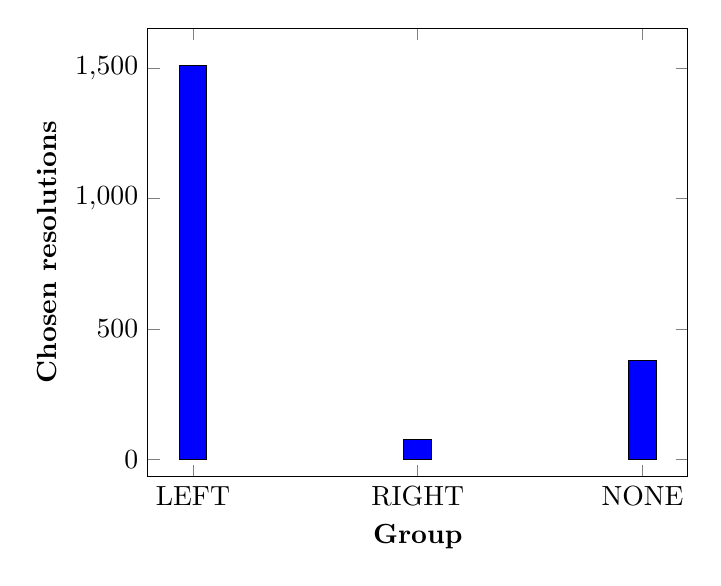
\begin{tikzpicture}
   \begin{axis}[
       symbolic x coords={LEFT, RIGHT, NONE},
       xtick=data,
       xlabel=\textbf{Group},
       ylabel=\textbf{Chosen resolutions}
     ]
       \addplot[ybar,fill=blue] coordinates {
           (LEFT,   1509)
           (RIGHT,  77)
           (NONE,   378)
       };
   \end{axis}
\end{tikzpicture}
\caption{Number of chosen resolutions for each group}\label{fig:groups}
\end{figure}

For cases where one of the versions was chosen completely, we can show that this chosen version ofter is the most recent version, as can be seen in Figure \ref{fig:recent}.

\begin{figure}
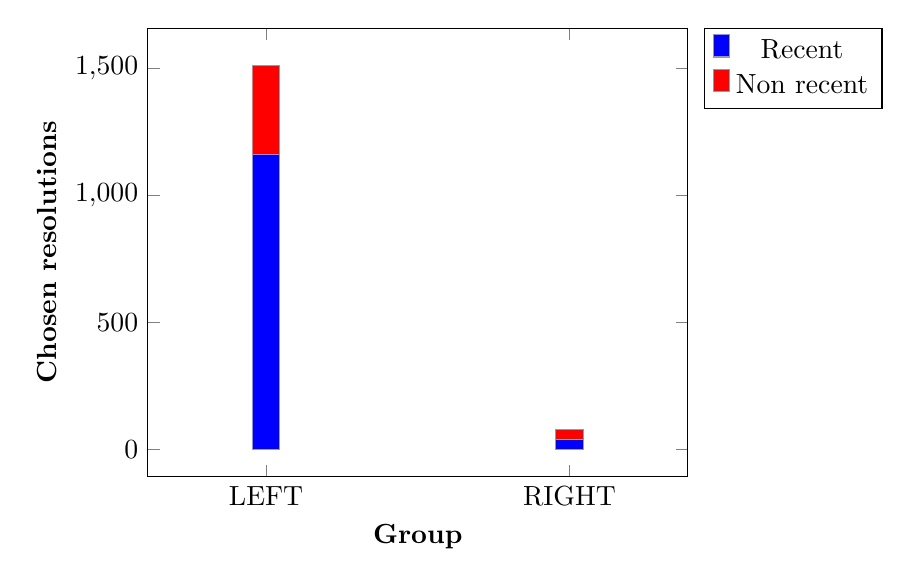
\begin{tikzpicture}
  \begin{axis}[ybar stacked,symbolic x coords={LEFT,RIGHT},xtick=data,enlarge x limits={abs=1.5cm},xlabel=\textbf{Group},ylabel=\textbf{Chosen resolutions},legend pos=outer north east]
      \addplot[black!40,fill=blue] coordinates
{(LEFT,1161)(RIGHT,40)};
      \addplot[black!40,fill=red]  coordinates
{(LEFT,348)(RIGHT,37)};
\legend{Recent, Non recent}
  \end{axis}
\end{tikzpicture}
\caption{Number of most recent versions chosen}\label{fig:recent}
\end{figure}

For some cases, the left and the right version differ in how many instances of specific keywords they contain. Figure \ref{fig:keywords} shows how often the version with most instances and the version with least instances of each keyword was chosen. \textit{Neither} means that the resolution is in the group \textit{None}, see Figure \ref{fig:groups}.

\begin{figure}
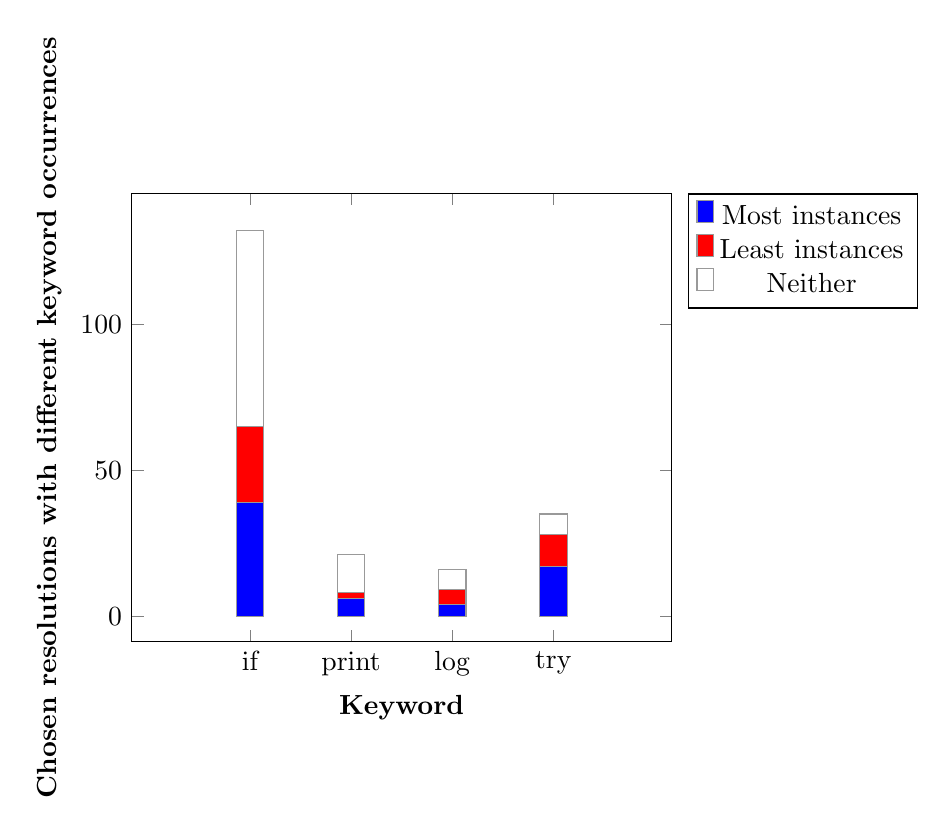
\begin{tikzpicture}
  \begin{axis}[ybar stacked,symbolic x coords={if,print,log,try},xtick=data,enlarge x limits={abs=1.5cm},xlabel=\textbf{Keyword},ylabel=\textbf{Chosen resolutions with different keyword occurrences},legend pos=outer north east]
      \addplot[black!40,fill=blue] coordinates{(if,39)(print,6)(log,4)(try,17)};
		\addplot[black!40,fill=red] coordinates{(if,26)(print,2)(log,5)(try,11)};
		\addplot[black!40,fill=white] coordinates{(if,67)(print,13)(log,7)(try,7)};
\legend{Most instances, Least instances, Neither}
  \end{axis}
\end{tikzpicture}
\caption{Number of chosen resolutions with different number of instances of keywords}\label{fig:keywords}
\end{figure}

Chart \ref{fig:setleft} and Chart \ref{fig:setright} show how often the left version and the right version is a superset or an intersection, and how often those versions are chosen as resolution.

\begin{figure}
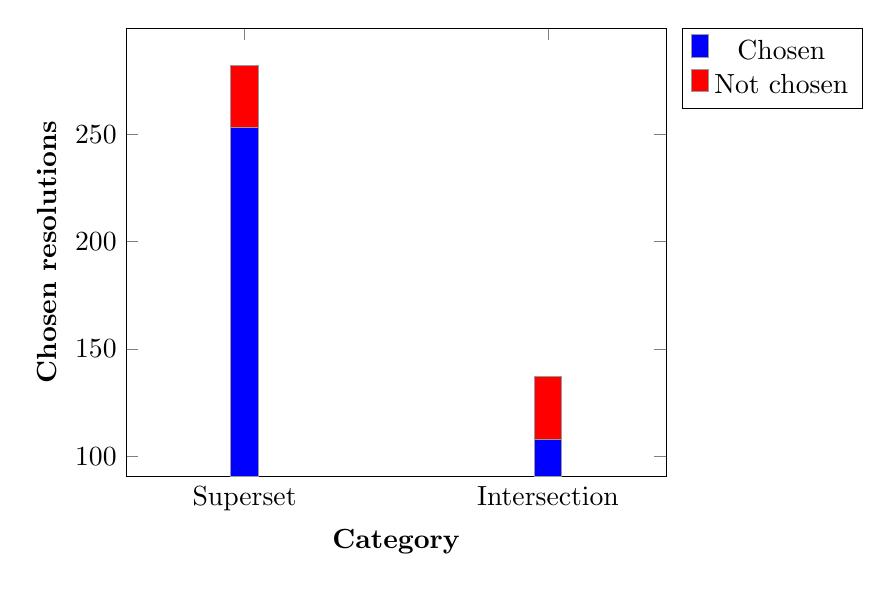
\begin{tikzpicture}
  \begin{axis}[ybar stacked,symbolic x coords={Superset,Intersection},xtick=data,enlarge x limits={abs=1.5cm},xlabel=\textbf{Category},ylabel=\textbf{Chosen resolutions},legend pos=outer north east]
      \addplot[black!40,fill=blue] coordinates{(Superset,253)(Intersection,108)};
      \addplot[black!40,fill=red] coordinates{(Superset,29)(Intersection,29)};
\legend{Chosen, Not chosen}
  \end{axis}
\end{tikzpicture}
\caption{Number of chosen left versions that are either a superset or an intersection}\label{fig:setleft}
\end{figure}

\begin{figure}
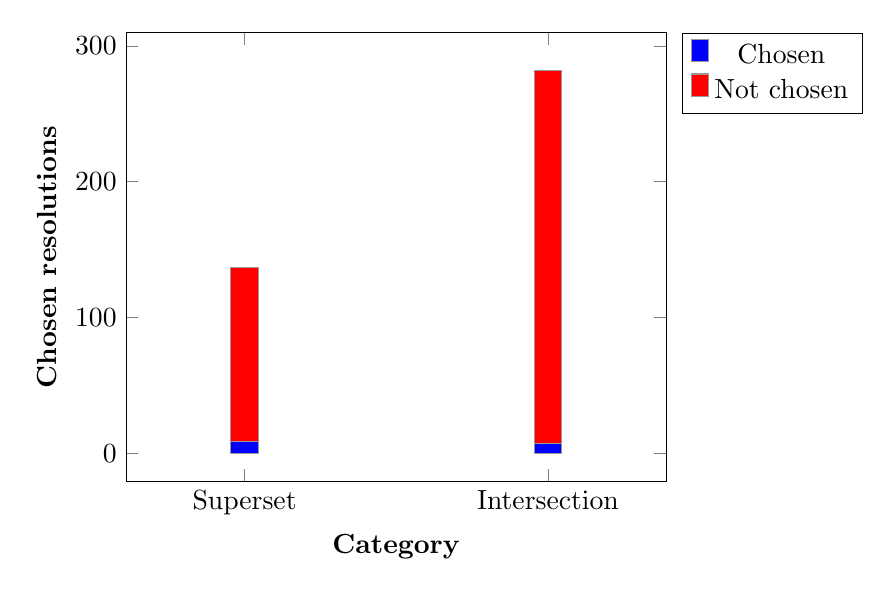
\begin{tikzpicture}
  \begin{axis}[ybar stacked,symbolic x coords={Superset,Intersection},xtick=data,enlarge x limits={abs=1.5cm},xlabel=\textbf{Category},ylabel=\textbf{Chosen resolutions},legend pos=outer north east]
      \addplot[black!40,fill=blue] coordinates{(Superset,9)(Intersection,7)};
      \addplot[black!40,fill=red] coordinates{(Superset,128)(Intersection,275)};
\legend{Chosen, Not chosen}
  \end{axis}
\end{tikzpicture}
\caption{Number of chosen right versions that are either a superset or an intersection}\label{fig:setright}
\end{figure}

\section{Discussion}
The most important result in this study is that in cases of conflicting code in methods or constructors in 3 out of 4 cases, developers tend to choose the left version when merging. The reasons for this is unclear, but there are two main scenarios; when pulling a remote branch and when merging a local branch into another one.

The left version is the commit that the developer who performs the merge has checked out when merging. If the conflicting merge is a result of pulling a remote branch, the left version is likely his own code, and the right version is someone else’s code. Table \ref{fig:recent} shows that the chosen version also often is the most recent version. This in combination with that the left version most often is chosen indicates that developers tend to choose their own code as resolution. This study has not gone into why developers resolve conflicts this way, but it might be interesting for future studies to investigate this further. If the conflicting merge is a result of merging a local branch into another one, the left version is the branch which the other branch was merged into.

Another interesting note about the results is that versions containing more of the keywords print and log are only chosen in about 1 out of 4 times. This might be because printouts and logging statements are removed at the time of the merge, when hopefully the newly implemented code is working as intended and tested, thus printouts and logs is no longer needed.
